\chapter{提案システム\label{sec:proposal_system}}
\thispagestyle{plain}

本章では,本研究で提案するシステムについて述べる.

\section{概要}

本研究で提案するシステムの構成を図\ref{fig:matching_system_big_arrow}に示す.
本システムは,対話雰囲気推定モジュール(Discordのボイスチャンネルからデータベースまでのフロー)とそれを用いたマッチング支援モジュール(データベース以降のフロー)から構築される.
本システムでは開催された作業通話の音声をBotによって取得し,対話雰囲気を推定したのちに,その他のメタデータと共に記録しそれらを用いた支援を行う.
主なユースケースは作業記録の可視化と募集ツイートの生成の二つである.
作業記録の可視化では,それまでに集めたユーザ自身の活動嗜好や活動雰囲気のデータの統計値や傾向を算出し表示する.
募集ツイートの生成では,条件を入力することで可視化された自身のデータとともに新しく開催する作業通話の参加者を募るためのツイートを生成する.

\begin{figure}
    \centering
    \fbox{
        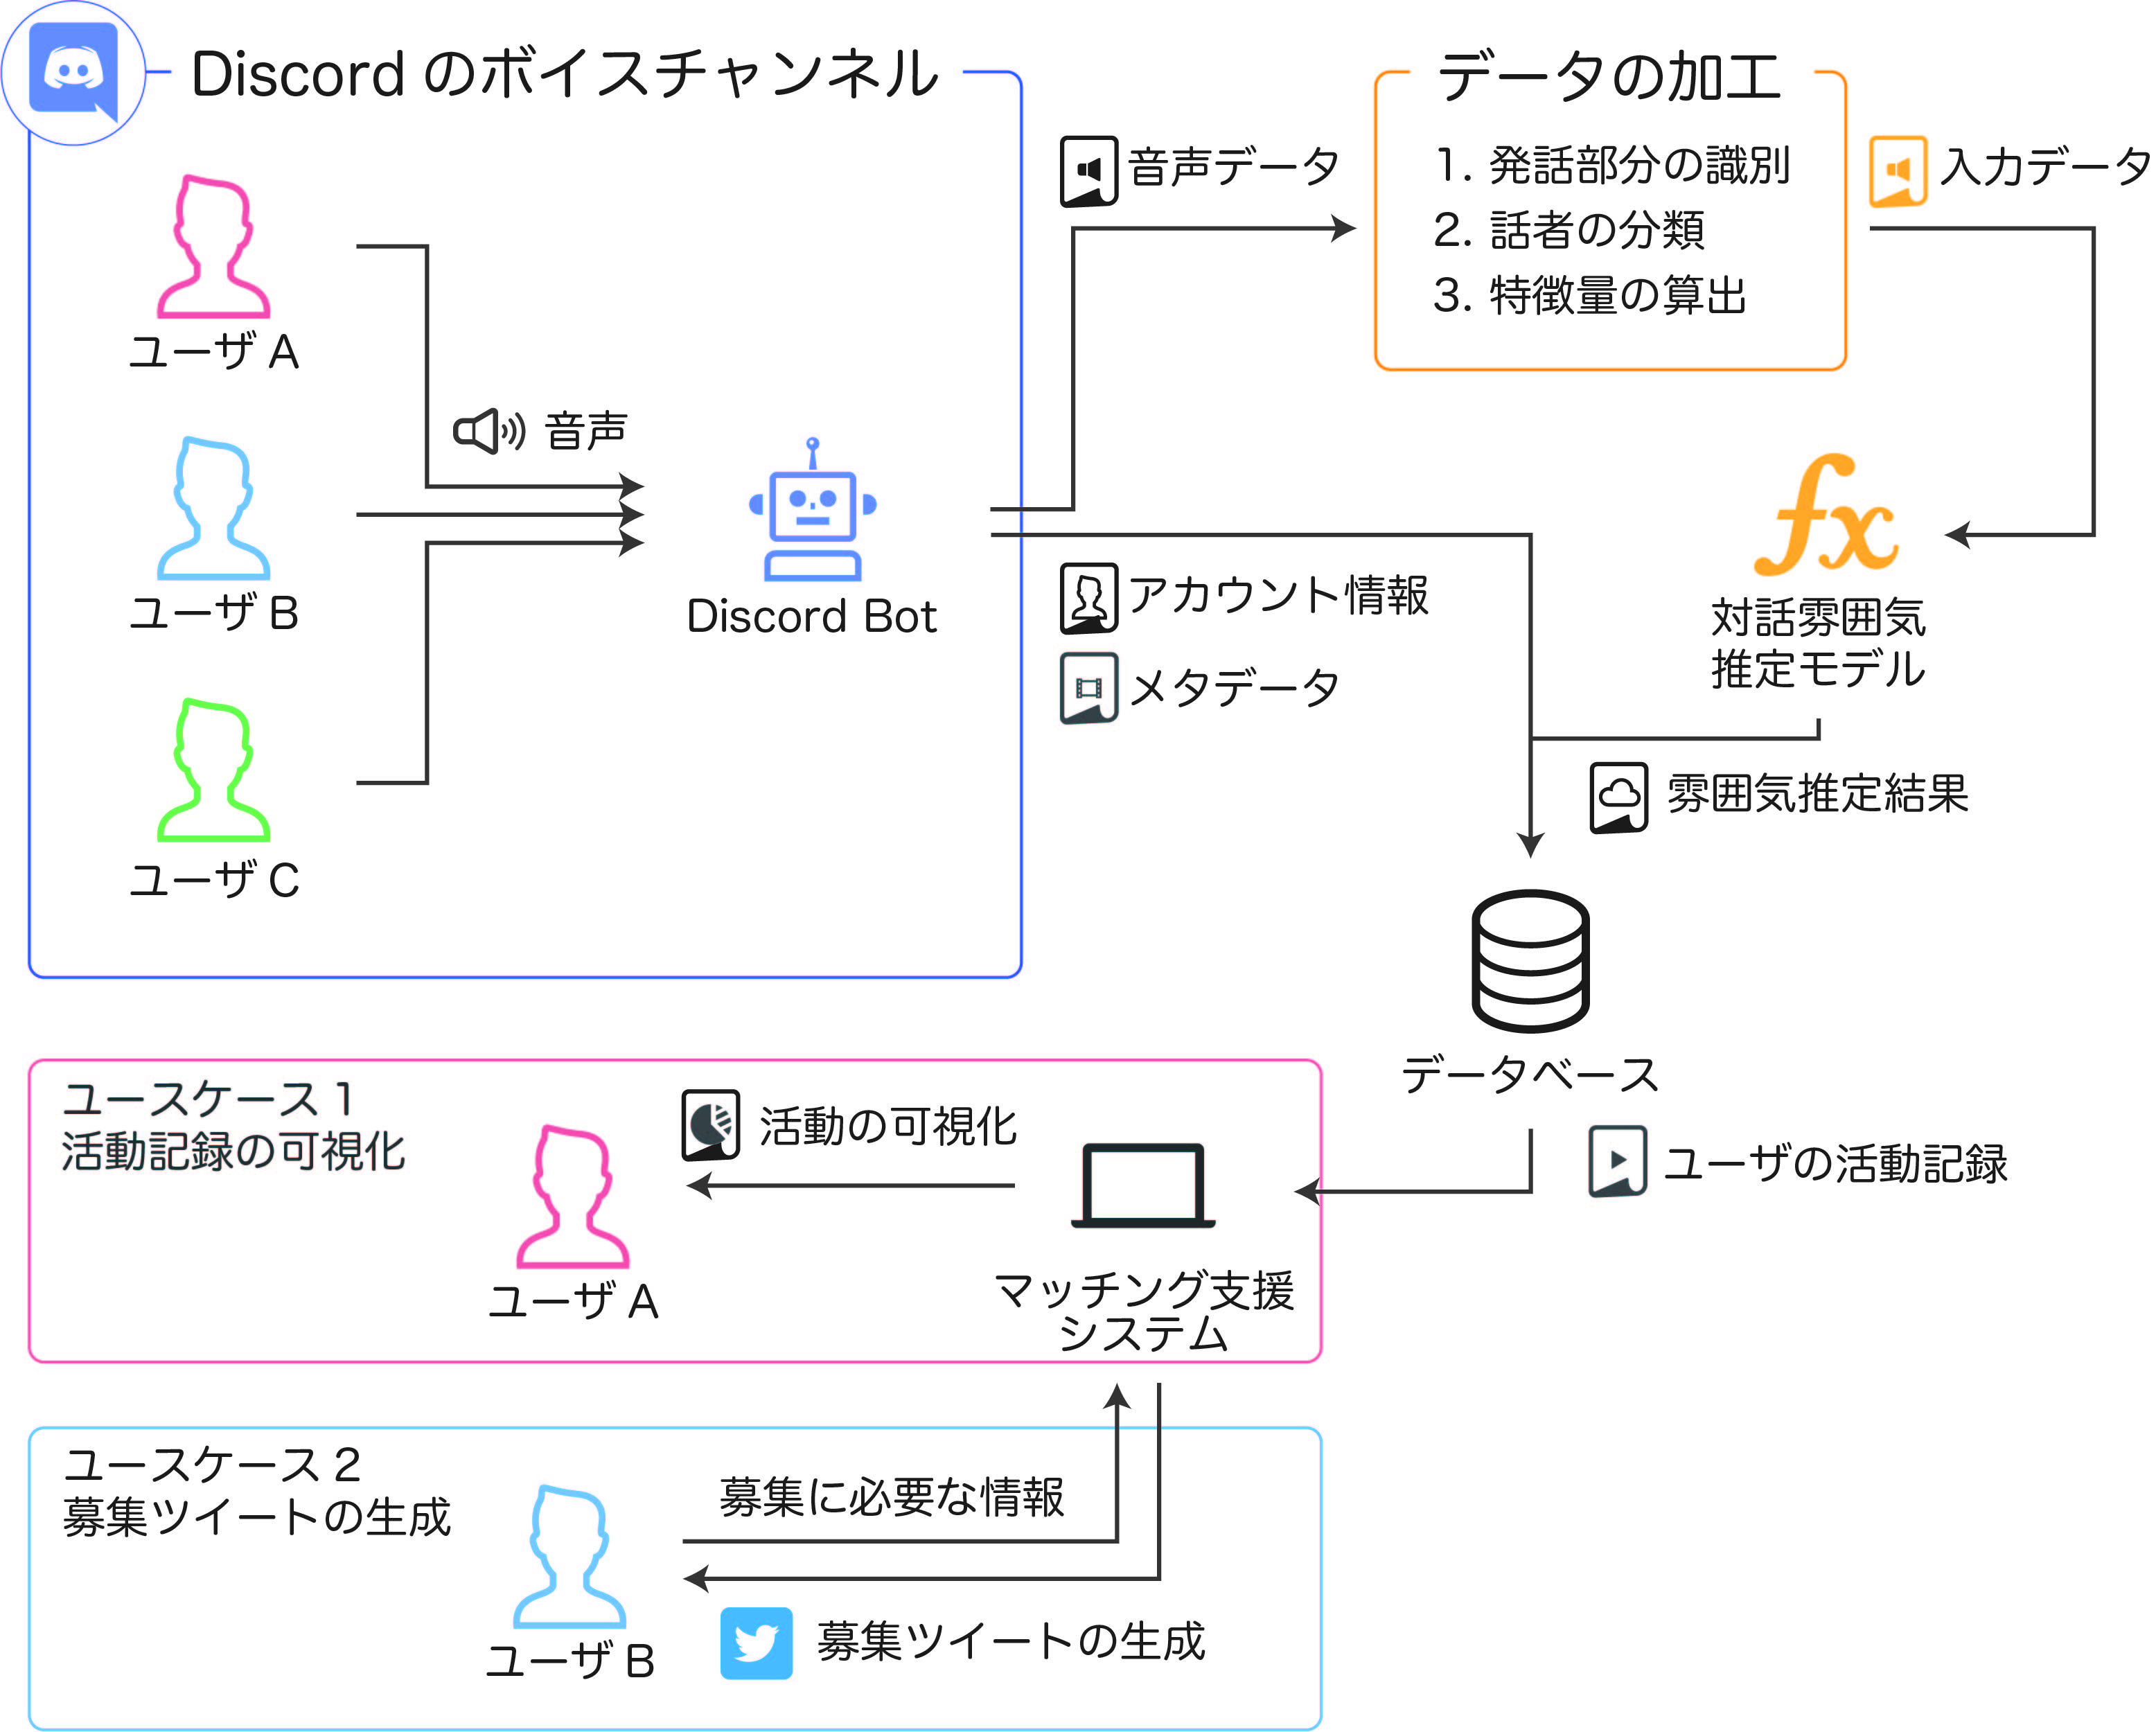
\includegraphics[width=0.7\textwidth]{figs/matching_system_big_arrow.jpg}
    }
    \caption{システムイメージ}
    \label{fig:matching_system_big_arrow}
\end{figure}

\section{対話雰囲気推定モジュール\label{node:estimation_module}}

本モジュールはDiscordで開催される作業通話を対象に,Botを作業通話に同席させBotを通して収集した情報から対話雰囲気を推定する.
対話雰囲気の推定には対話雰囲気に関する特徴量を学習した対話雰囲気推定モデルを用いる.対話雰囲気推定モデルの構築については第\ref{sec:estimation_model}章で詳細に述べる.

本モジュールでは,対話雰囲気推定のために音声データの収集を行う.
しかし,本研究で構築する対話雰囲気推定モデルでは言語情報を用いないため,誰がどのタイミングでどの程度発話したのかを基に算出した特徴量(以下,「発話時間特徴量」)のみを収集する.
これは第\ref{sec:related_researchs}章で述べた豊田らの手法を参考にしており,参加者のプライバシーに配慮しながらも高精度の推定を行えることから採用した.

Botの利用方法の想定を示す.
まず,Botはサーバに招待されることで利用可能状態となる.
作業通話を開始した際に開始用のコマンドをBotに対して入力することで録音を開始する.
作業通話が終了した際に終了用のコマンドを入力することで録音の停止と対話雰囲気の推定結果の出力をテキストチャンネル上に行う.
ユーザはそれを見て推定雰囲気の確認や主観的に正しいと感じた雰囲気への修正を行える.
それらのデータはサーバに記録される.記録したデータは再び学習データとしてモデルの精度向上に利用することを想定している.

\section{マッチング支援モジュール}

本モジュールは,3.1節のモジュールによって推定された対話雰囲気を用いてSNS募集及びその募集への参加の支援を行う.
本モジュールの対象はTwitterでのSNS募集である.
本モジュールは3.1節のモジュールより得た対話雰囲気推定結果と,募集を行うユーザの開催したい作業通話の概要の入力を行うことで募集用の投稿(図\ref{fig:tweet_image})を生成することを主機能としている.
本機能によって生成される投稿には,作業内容や開催時間帯,募集人数,これまでどのような雰囲気で活動する傾向があったかなどを掲載する.
また,次に示す作業嗜好の可視化機能によって可視化された作業嗜好も併せて掲載する.
本機能は,一目で無縁ユーザ向けの募集文であることがわかることと,開催したい作業通話の概要がわかることによって明確で効率的な募集形態を目指している.

\begin{figure}
    \centering
    \fbox{
        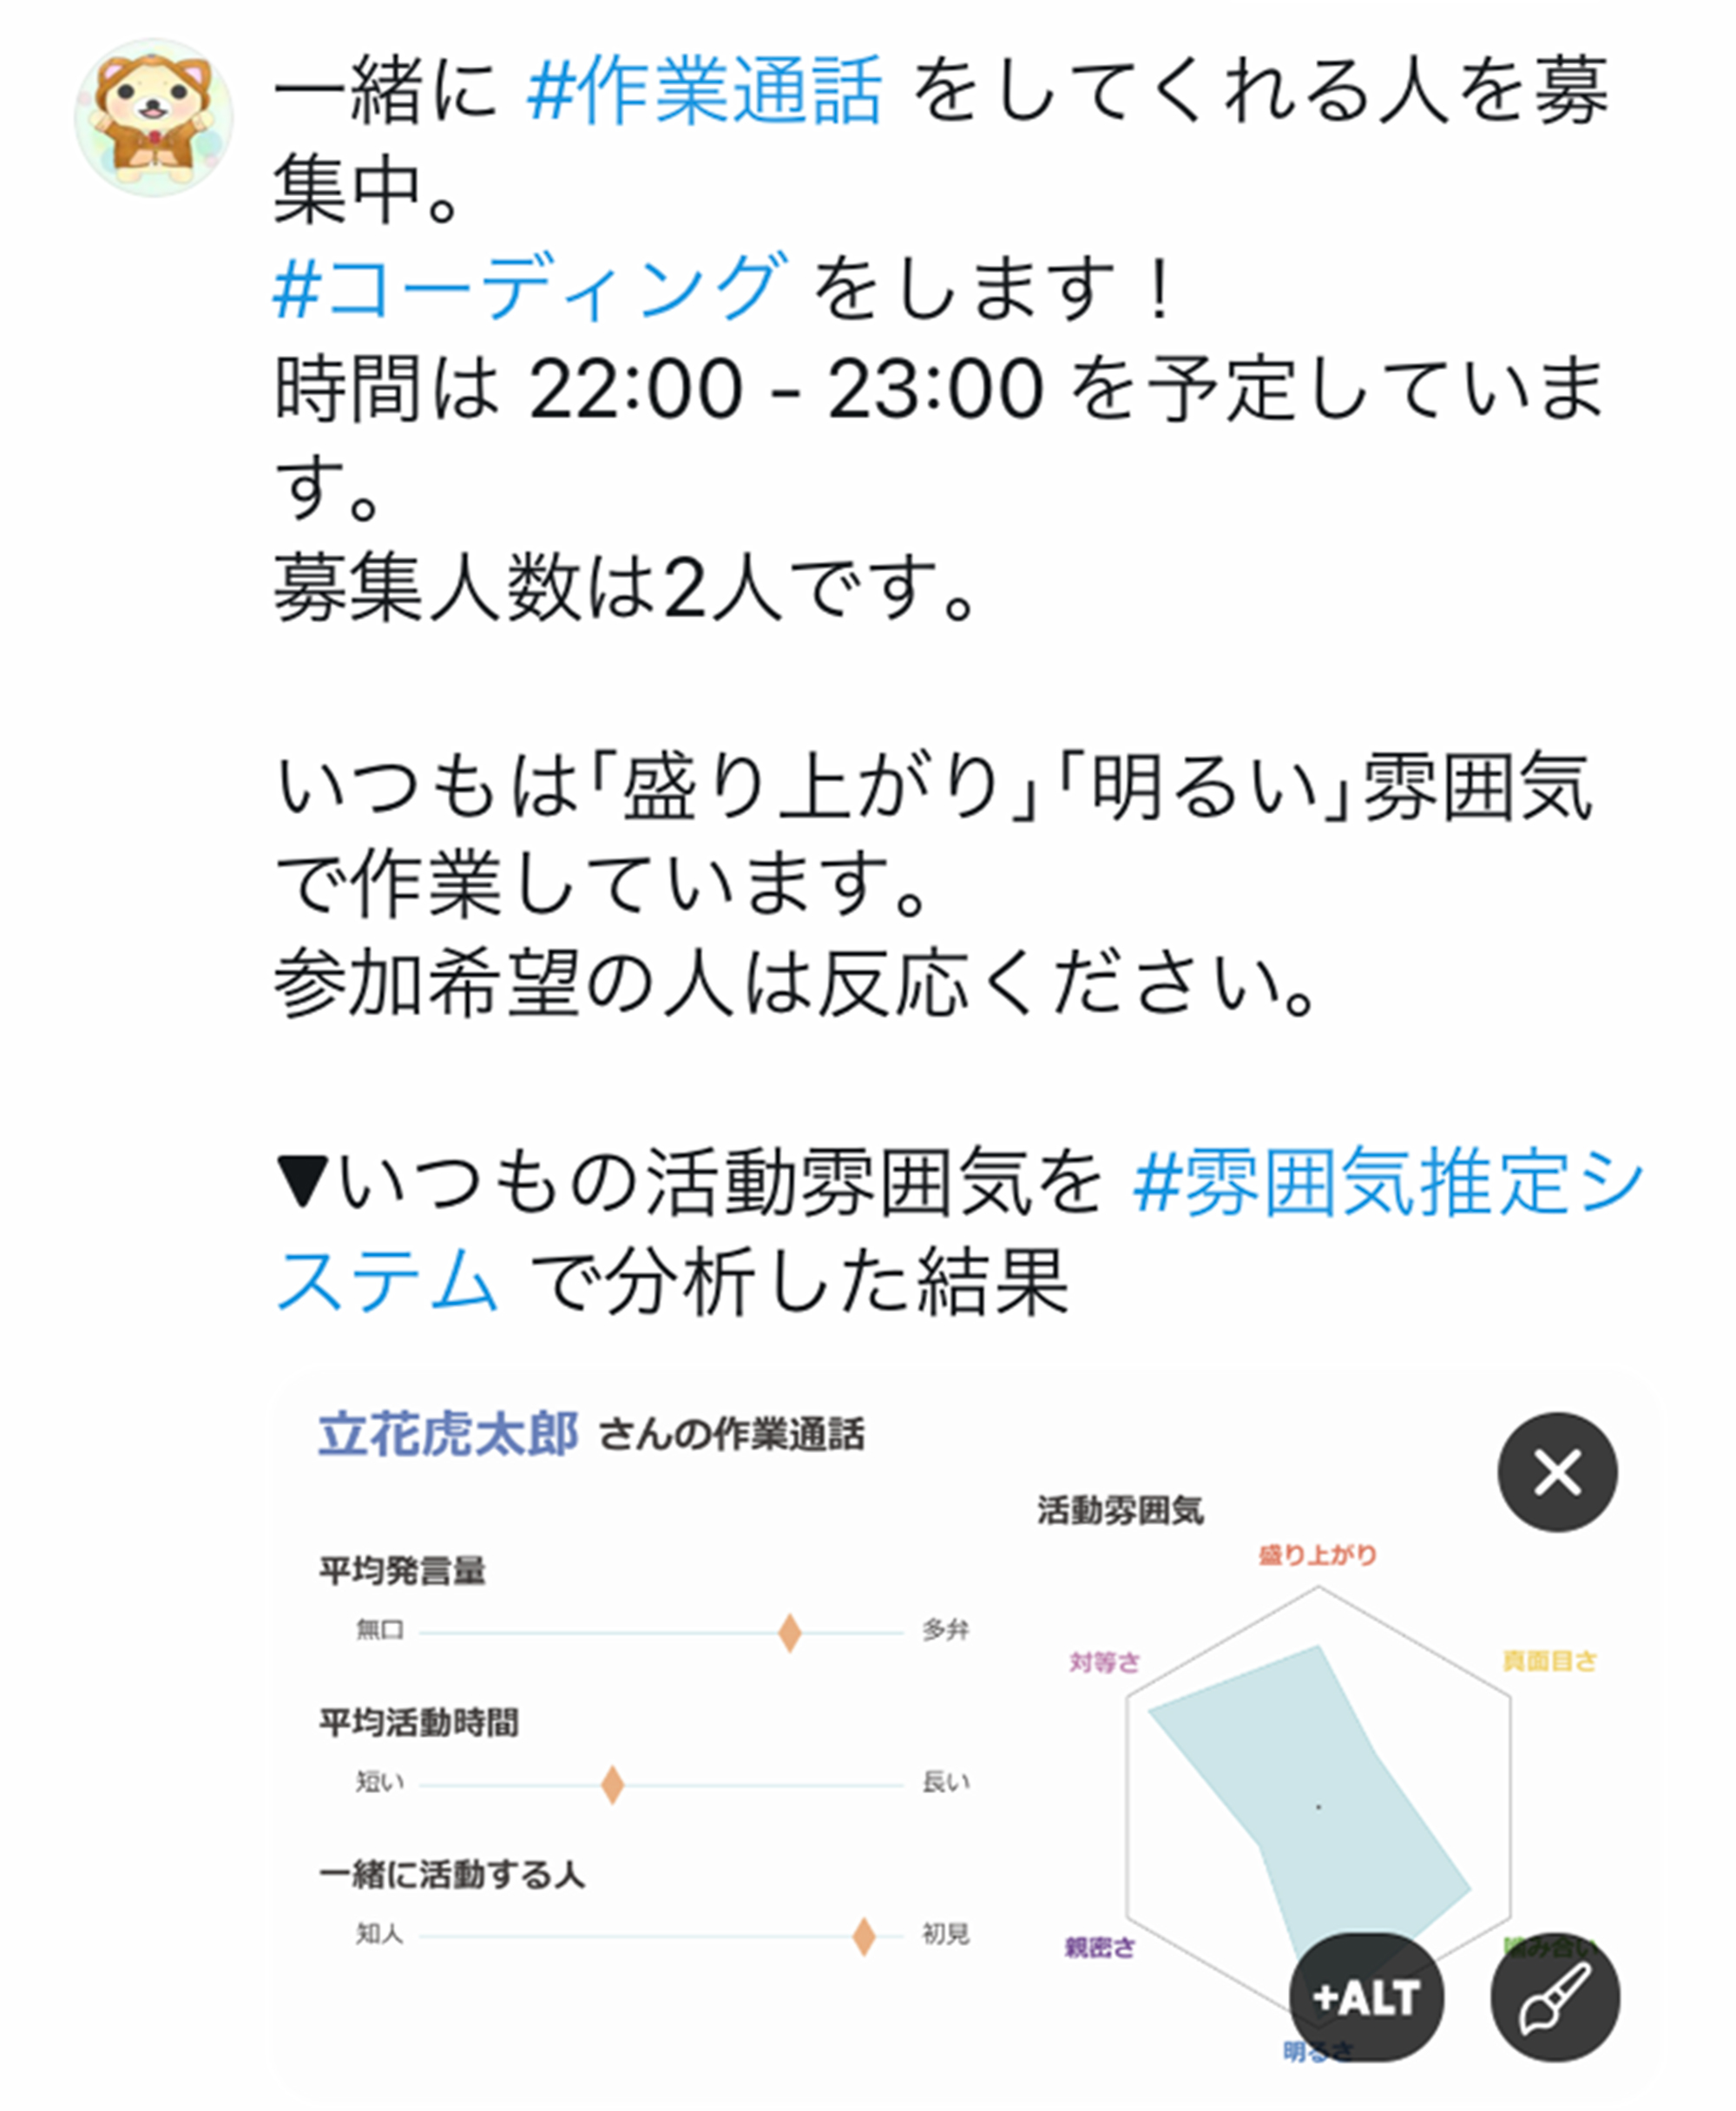
\includegraphics[width=0.7\textwidth]{figs/tweet_image.jpg}
    }
    \caption{生成する投稿のイメージ}
    \label{fig:tweet_image}
\end{figure}

本モジュールには作業嗜好の可視化機能の実装を行う(図\ref{fig:estimationgraph}).
本機能は前述した募集投稿に掲載する情報を可視化する機能である.
表示する情報は,推定された対話雰囲気の傾向値,作業時間長の平均値,雑談量の平均値,他の参加者の傾向値である.
推定された対話雰囲気の傾向値とは盛り上がっている雰囲気の対話が多いことなどをレーダーチャートにて表現した値を指し,他の参加者の傾向値とはどの程度初対面の人と積極的に作業通話を開催しているかを指す.

\begin{figure}
    \centering
    \fbox{
        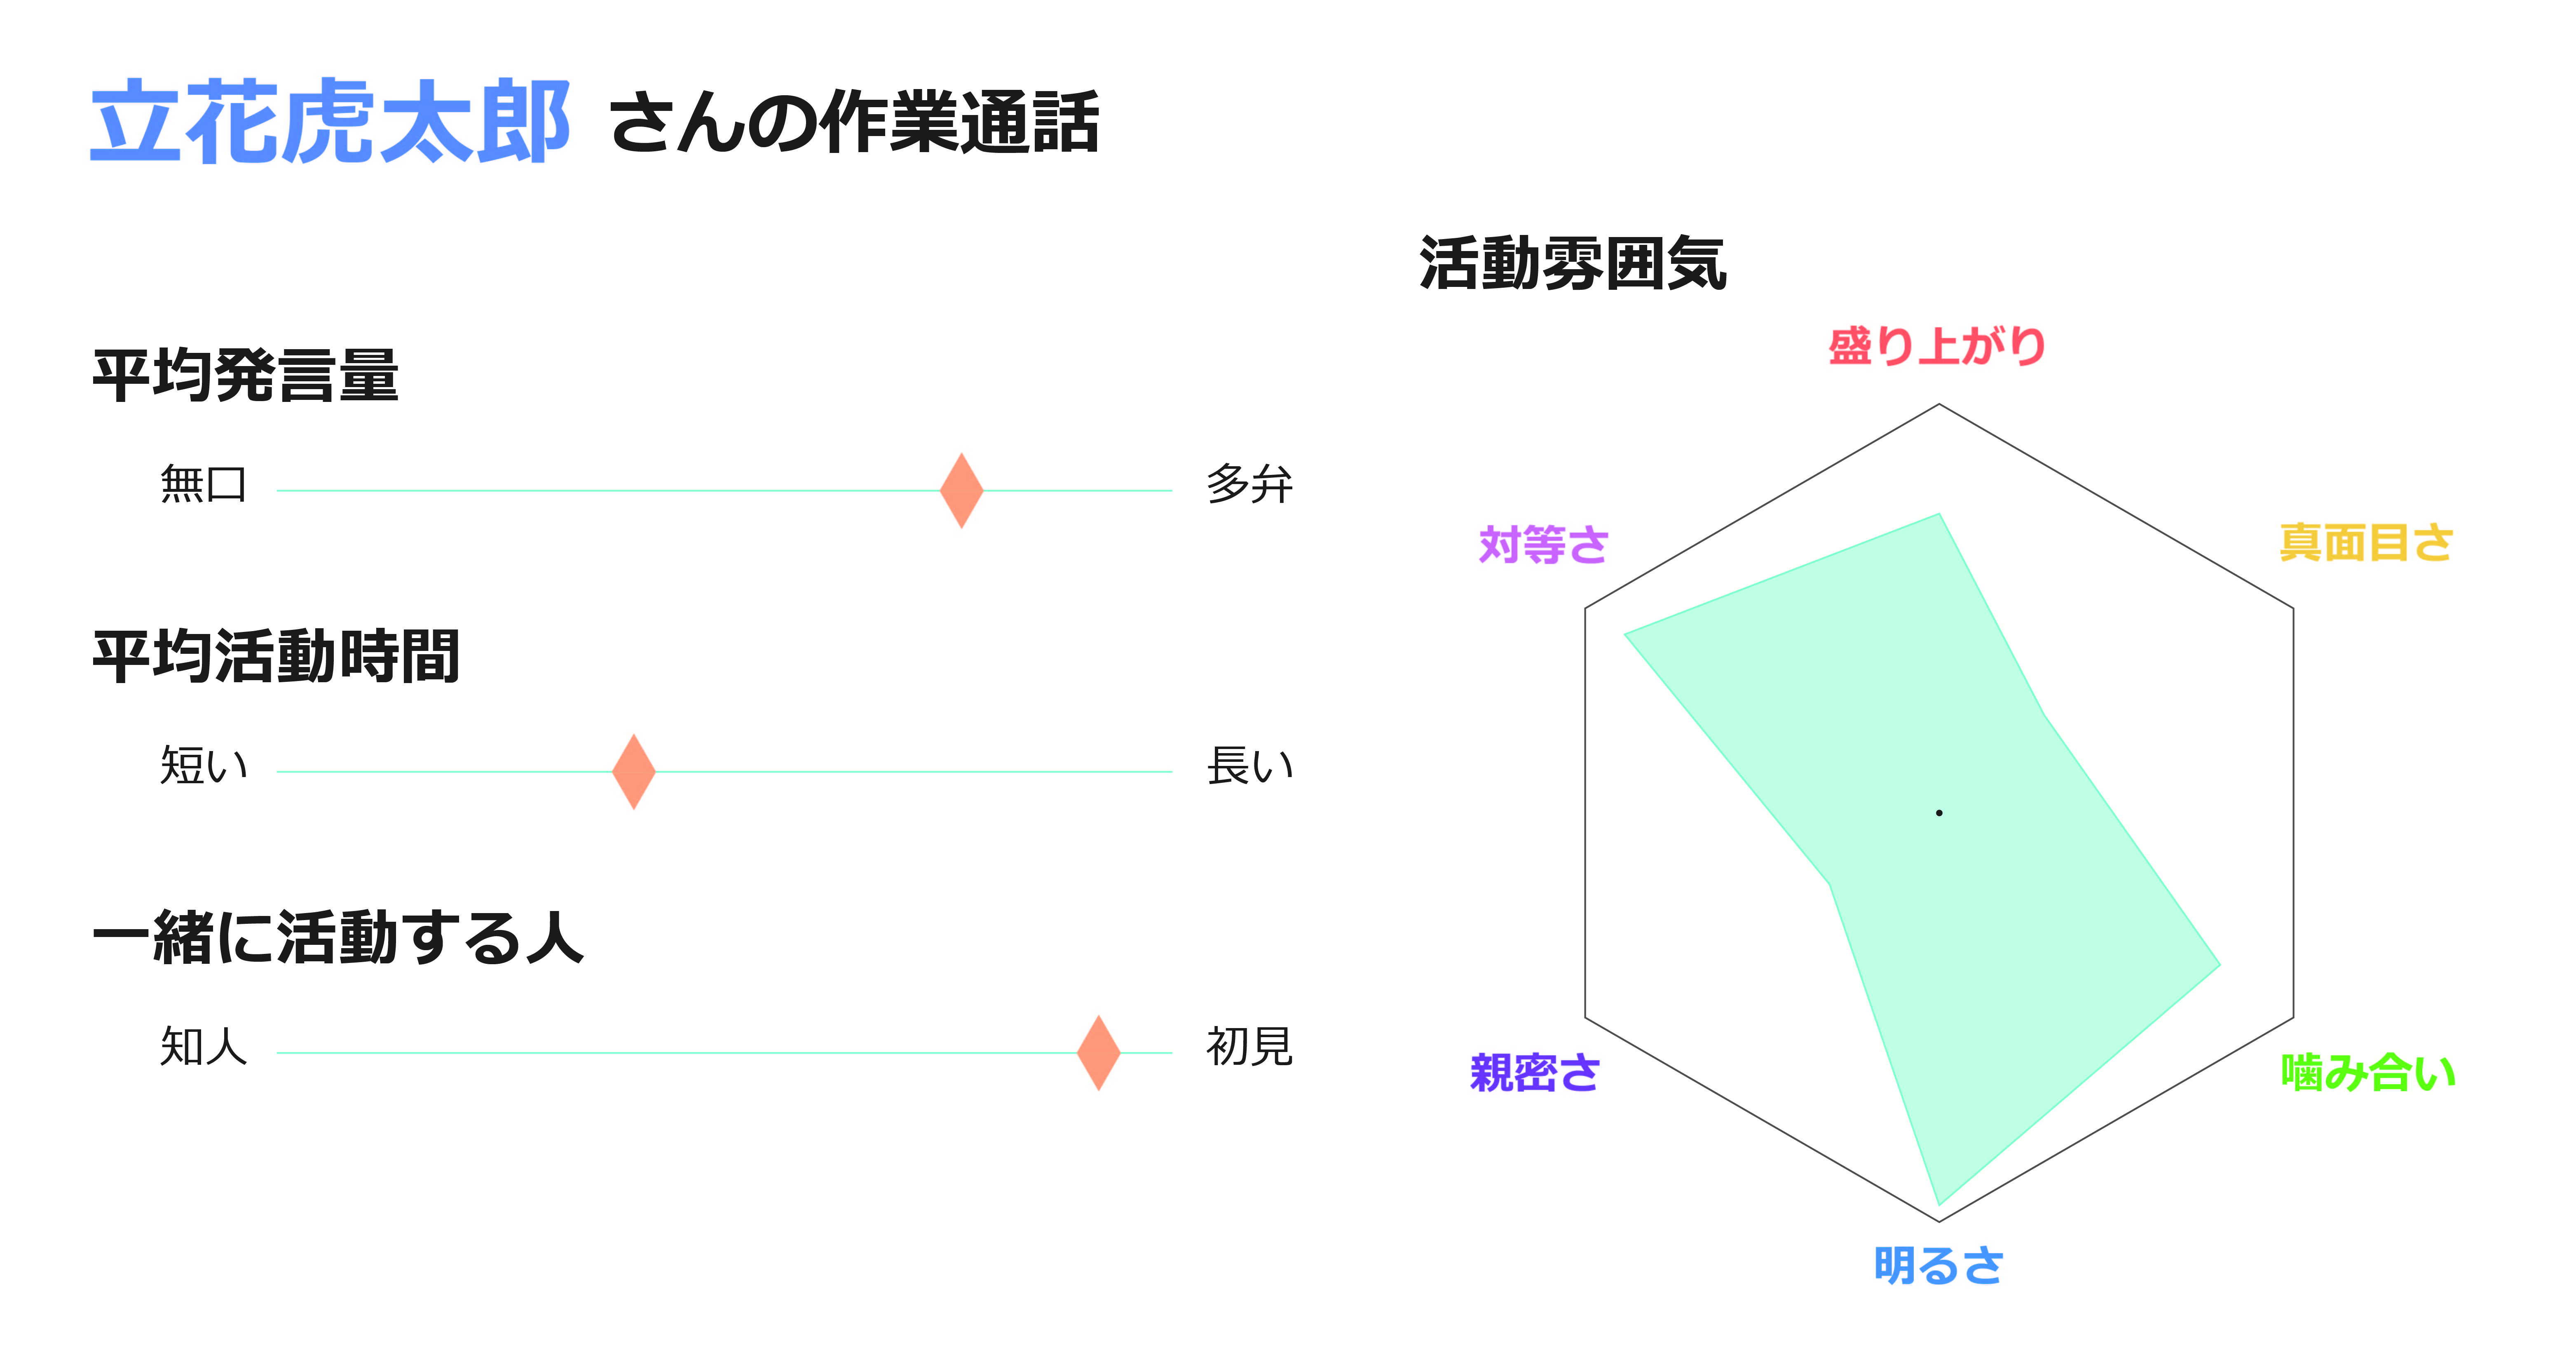
\includegraphics[width=0.7\textwidth]{figs/estimationgraph.jpg}
    }
    \caption{作業嗜好の可視化イメージ}
    \label{fig:estimationgraph}
\end{figure}

将来的には,本モジュールを用いて作業嗜好の合うユーザの推薦等無縁ユーザとの繋がり形成の機会を増加させる枠組みの構築を目指す.
